%!Tex Program = xelatex
\documentclass[a4paper]{article}
\usepackage{fontspec, xunicode, xltxtra}
\usepackage[slantfont,boldfont]{xeCJK} % 允许斜体和粗体
\usepackage{geometry}
\usepackage{indentfirst}
\usepackage{lastpage}
\usepackage{multirow}
\usepackage{multicol}
\usepackage{titlesec}
\usepackage{enumerate}
\usepackage{booktabs}
\usepackage{extarrows}
\usepackage{fancyhdr,fancybox}
\usepackage[table]{xcolor}
\usepackage{float}
\usepackage{tikz}
%\usepackage{amssymb}
%\usepackage{amsmath}
%\usepackage{caption}
%\usepackage{dirtree}
%\usepackage{algorithm}
%\usepackage{algpseudocode}
\usepackage{listings}
\usepackage[colorlinks,linkcolor=black]{hyperref}

\geometry{left=2.5cm,right=2.5cm,top=2.5cm,bottom=2.5cm}

%cmd “fc-list :lang=zh-cn”
\defaultfontfeatures{Mapping=tex-text}
\setmainfont{Book Antiqua}   % 英文衬线字体 Times New Roman, Palatino Linotype
\setmonofont{Consolas}   % 英文等宽字体 Monaco
\setsansfont{Consolas} % 英文无衬线字体 Arial, Futura, Optima
\setCJKmainfont{SimSun}   % 设置缺省中文字体
\setCJKmonofont{FangSong}   % 设置等宽字体
\setCJKsansfont{SimHei}   % 设置无衬线字体 Microsoft YaHei

\newfontfamily\timesroman{Times New Roman}
\newfontfamily\consolas{Consolas}

\newfontfamily\ensong{SimSun}
\newfontfamily\enhei{SimHei}
\newfontfamily\enyahei{Microsoft YaHei}
\newfontfamily\palatino{Palatino Linotype}
\newfontfamily\nimbus{Nimbus Sans L}
\newfontfamily\enkai{STKaiti}
\newfontfamily\enfangsong{FangSong}
\newfontfamily\akaDora[Path=../]{akaDora.ttf}

\setCJKfamilyfont{song}{SimSun}
\newcommand{\song}{\CJKfamily{song}\ensong}
\setCJKfamilyfont{heiti}{SimHei}
\newcommand{\heiti}{\CJKfamily{heiti}\enhei}
\setCJKfamilyfont{yahei}{Microsoft YaHei}
\newcommand{\yahei}{\CJKfamily{yahei}\enyahei}
\setCJKfamilyfont{kaiti}{STKaiti}
\newcommand{\kaiti}{\CJKfamily{kaiti}\enkai}
\setCJKfamilyfont{fangsong}{FangSong}
\newcommand{\fangsong}{\CJKfamily{fangsong}\enfangsong}

\XeTeXlinebreaklocale "zh"
\XeTeXlinebreakskip = 0pt plus 1pt minus 0.1pt

\titlespacing*{\chapter} {0pt}{50pt}{40pt}
\titlespacing*{\section} {0pt}{3.5ex plus 1ex minus .2ex}{2.3ex plus .2ex}
\titlespacing*{\subsection} {0pt}{3.25ex plus 1ex minus .2ex}{1.5ex plus .2ex}
\titlespacing*{\subsubsection}{0pt}{3.25ex plus 1ex minus .2ex}{1.5ex plus .2ex}
\titlespacing*{\paragraph} {0pt}{3.25ex plus 1ex minus .2ex}{1em}
\titlespacing*{\subparagraph} {\parindent}{3.25ex plus 1ex minus .2ex}{1em}

\titleformat{\section}{\Large \bf \nimbus}{\thesection}{1em}{}
\titleformat{\subsection}{\large \bf \nimbus}{\thesubsection}{0.5em}{}

\setlength{\parskip}{0.5\baselineskip}
\setlength{\abovedisplayskip}{1pt}
\setlength{\belowdisplayskip}{1pt}

\usetikzlibrary{arrows,positioning}
\newcommand\nbvspace[1][3]{\vspace*{\stretch{#1}}}
\newcommand\nbstretchyspace{\spaceskip0.5em plus 0.25em minus 0.25em}
\newcommand{\nbtitlestretch}{\spaceskip0.6em}

\pagestyle{fancy}


\lstset{
    basicstyle=\small,
    backgroundcolor=\color{white},
    %keywordstyle=\color{keywordcolor}\bfseries, %\underbar,
    keywordstyle=\color{blue}\bfseries,
    %morekeywords={*,keyword_a,keyword_b},
    sensitive=true,
    identifierstyle=\small,
    showspaces=false,
    showstringspaces=false,
    showtabs=false,
    tabsize=4,
    frame=single,
    commentstyle=\color{olive} \textit,
    stringstyle=\ttfamily,
    showstringspaces=false,
    captionpos=b,
    breaklines=true,
    breakatwhitespace=true,
  }

\lstdefinelanguage{Makefile} {
  numberblanklines=false,
  keywordstyle=\color{blue}\bfseries,
  morekeywords={gedit,ls,rm,source,sudo,tar},
}

\lstdefinelanguage{LinuxTerminal} {
  numberblanklines=false,
  keywordstyle=\color{blue}\bfseries,
  morekeywords={cat,cd,chmod,gedit,ln,ls,
    make,mkdir,rm,source,sudo,tar,touch},
  morecomment=[l]{\#},
}

\lstdefinelanguage{PlainText} {
  numberblanklines=false,
}



\usepackage{tikz}

\begin{document}
  \thispagestyle{empty}
  \begin{center}
    \bfseries
    \nbvspace[2]
    \begin{figure}[H]
      \centering
      
\includegraphics[width=0.6\textwidth]{../logo.pdf}
    \end{figure}
    {\Huge GDPLS Movie} \\[10pt]
    {\LARGE\akaDora Grand Duke of Programming Language Script}\\[10pt]
    {\Huge 2017 June} \\
    \nbvspace[1]
    \Huge Investigation Report\\
    \nbvspace[1]
    \normalsize Generated \& Compiled By \XeLaTeX
    \nbvspace[3]
  \end{center}
  \newpage

  \lhead{\emph{VISION TABLE}}
  \begin{table}[H]
    \centering
    \renewcommand\arraystretch{1.3}
    \rowcolors{2}{blue!50}{blue!20}
    \begin{tabular}{lllp{28em}}
      %\rowcolors{1}{blue!80}{blue!10}
      \multicolumn{4}{c}{\heiti 版本日志}\\
      版本号 & 修改人 & 修改时间 & \multicolumn{1}{c}{说明} \\
      1.0.0 & 方铭 & 2016.5.6 & 根据第一次会议内容制定调查问卷初稿\\
      1.1.0 & 方铭 & 2016.6.1 & 更改封面\\
      &&&\\
      &&&\\ % span text width
    \end{tabular}
  \end{table}
  \newpage
  \lhead{\emph{调查报告}}
  
\section{调查目标}
启动本项目之前,为确定开发平台以及产品亮点,我们首先通过线上调查问卷的形式,
针对目标用户(以大学生群体为主)进行了初步的需求分析。
\section{问卷题目}
为了降低产品风险,明确用户需求,我们设计了以下这些问题:\\[10pt]
\def\ind{\indent }
1. 您的年龄是:\\
\ind A.18 岁以下\\
\ind B.18-25 岁\\
\ind C.25-35 岁\\
\ind D.35 岁以上\\[7pt]
2 .您是否有去电影院看电影的习惯: \\
\ind A.经常看,每年观影 6 次以上\\
\ind B.看,每年观影 4-6 次\\
\ind C.偶尔看,每年观影 1-3 次\\
\ind D.没有看电影的习惯\\[7pt]
3 .您是否有通过网络渠道购买电影票:\\
\ind A.否,在电影院现场原价购票\\
\ind B.否,通过会员卡购票\\
\ind C.是,通过团购网站团购\\
\ind D.是,通过在线选座购票\\[7pt]
4 .什么因素吸引您通过网络在线选座购票(多选题):\\
\ind A.网络选择购票经常会有优惠\\
\ind B.在线选座免去现场排队,不用等位\\
\ind C.不同于团购针对有些影片还要另外加钱\\
\ind D.智能手机以及 4G 网络的普及使得网络购票可以随时随地\\[7pt]
5 .你使用过以下哪几种网络购票软件(多选题):\\
\ind A.猫眼电影\\
\ind B.淘宝电影\\
\ind C.微信电影票\\
\ind D.百度糯米\\
\ind E.格瓦拉\\
\ind F.时光网\\
\ind G.其他\\[7pt]
6 .你是否会固定使用同一款购票软件:\\
\ind A.是的,习惯性购票\\
\ind B.不会,一般会对比价格找最便宜的\\
\ind C.不一定,但会选择比较大型的平台购票\\
\ind D.不一定,要看哪个 app 做的活动对我有吸引力\\[7pt]
7 .哪个是影响你选择一款软件购票最主要的原因:\\
\ind A.软件知名度\\
\ind B.电影票是否可改签或者退票\\
\ind C.软件的售票价格\\
\ind D.软件的多功能性\\[7pt]
8 .多少差价会令你换一个软件并且新注册一个账号购票\\
\ind A.0-5 元\\
\ind B.6-10 元\\
\ind C.11-15 元\\
\ind D.15 元以上\\[7pt]
9 .什么因素决定你是否会再次使用网络在线购票:\\
\ind A.持续有优惠的价格\\
\ind B.软件支付等流程便捷\\
\ind C.精彩的活动推送\\
\ind D.人性化的服务\\
\ind F.不用现场等位,网络选择提供了便捷\\[7pt]
10. 你最希望现在的在线 电影\\
\underline{\hspace{10cm}\ }

\section{调查报告}
\begin{enumerate}
  \item 从问卷收集结果来看,我们本次调查问卷的对象主要聚集在 18 岁到 25 岁之间,所以下
面的结论主要是针对这一年年龄段的群体,主要是大学生等年轻人,也说明了对在线电影购
票这种方式来说,在大学生中更在普及以及受欢迎。
\begin{figure}[H]
  \centering
  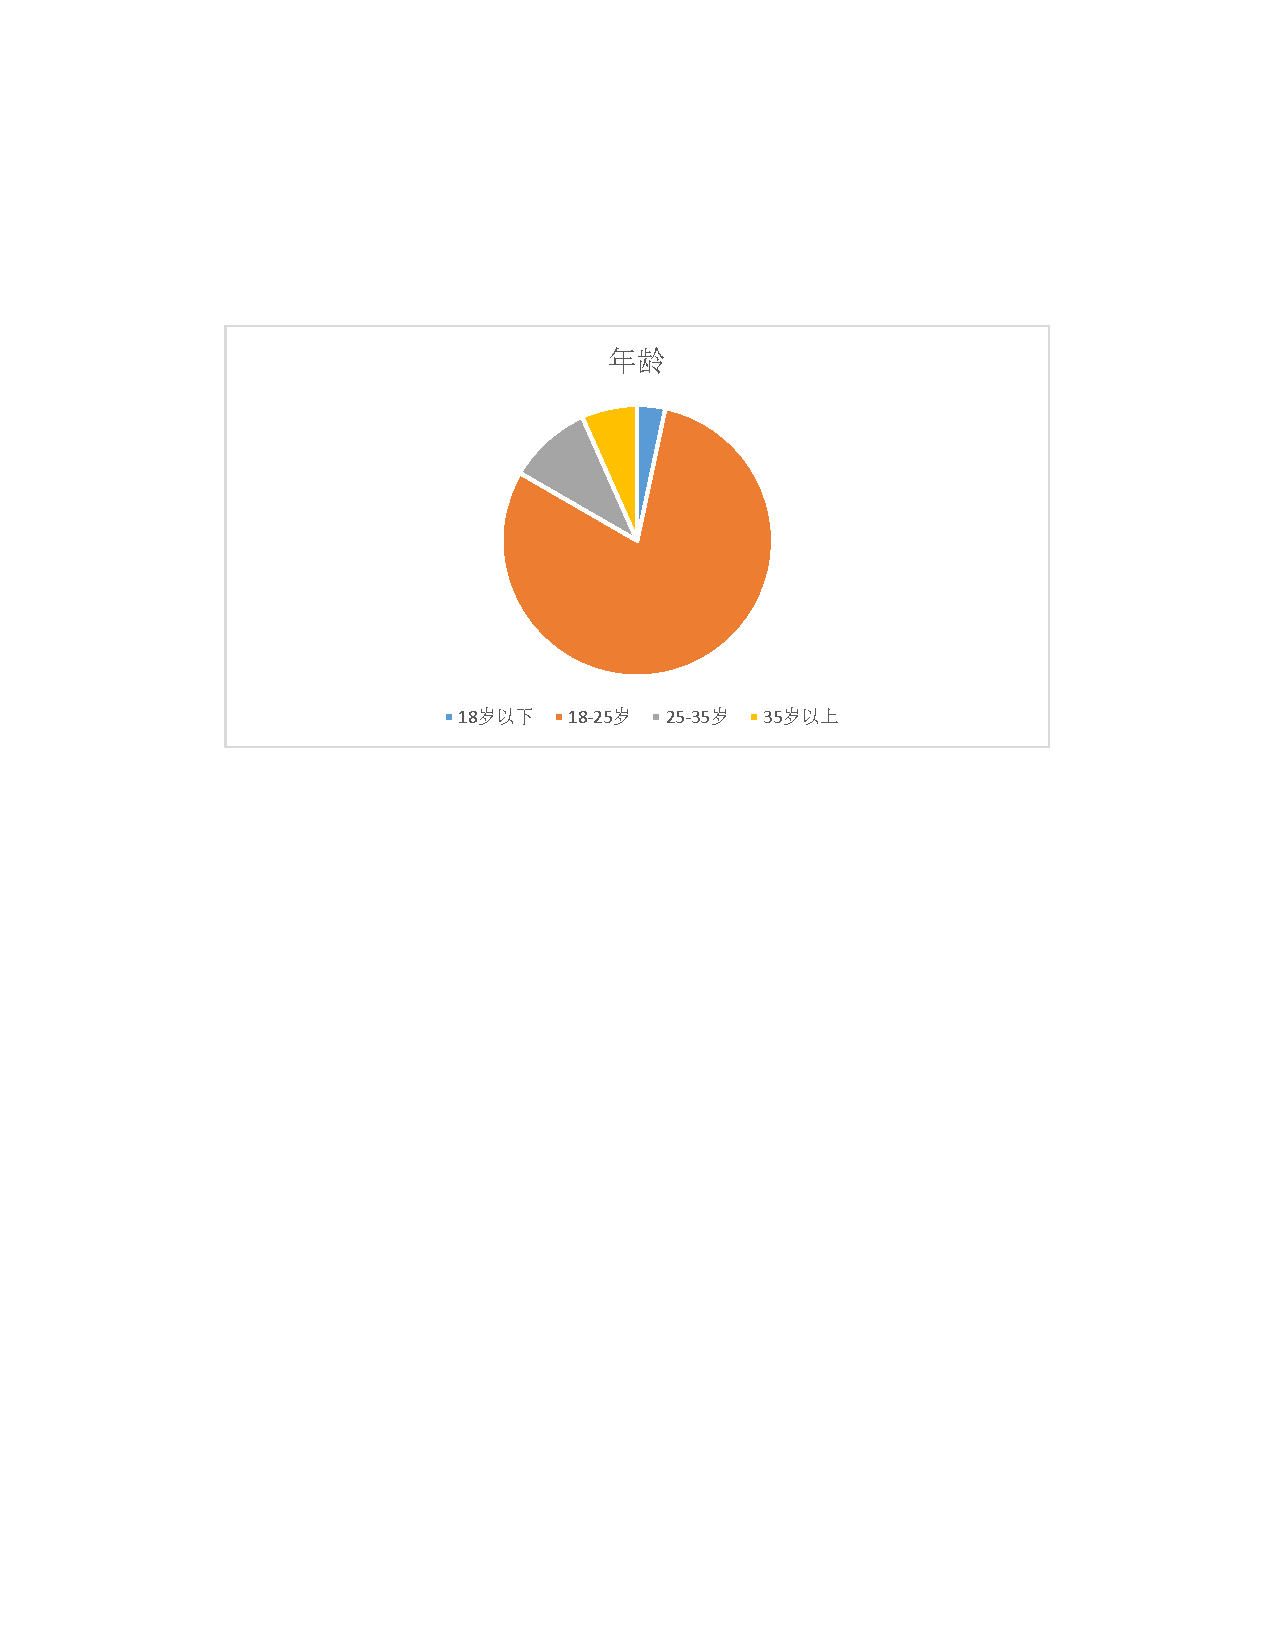
\includegraphics[width=0.6\textwidth]{figure/1.pdf}
%  \caption{}
\end{figure}
  \item 从结果上来看,在现在的社会环境下,大部分人都开始有了去电影院看电影的习惯,而
且其中有大部分人已经开始对电影院看电影这种娱乐消遣的方式有了一定的频度和习惯性。
\begin{figure}[H]
  \centering
  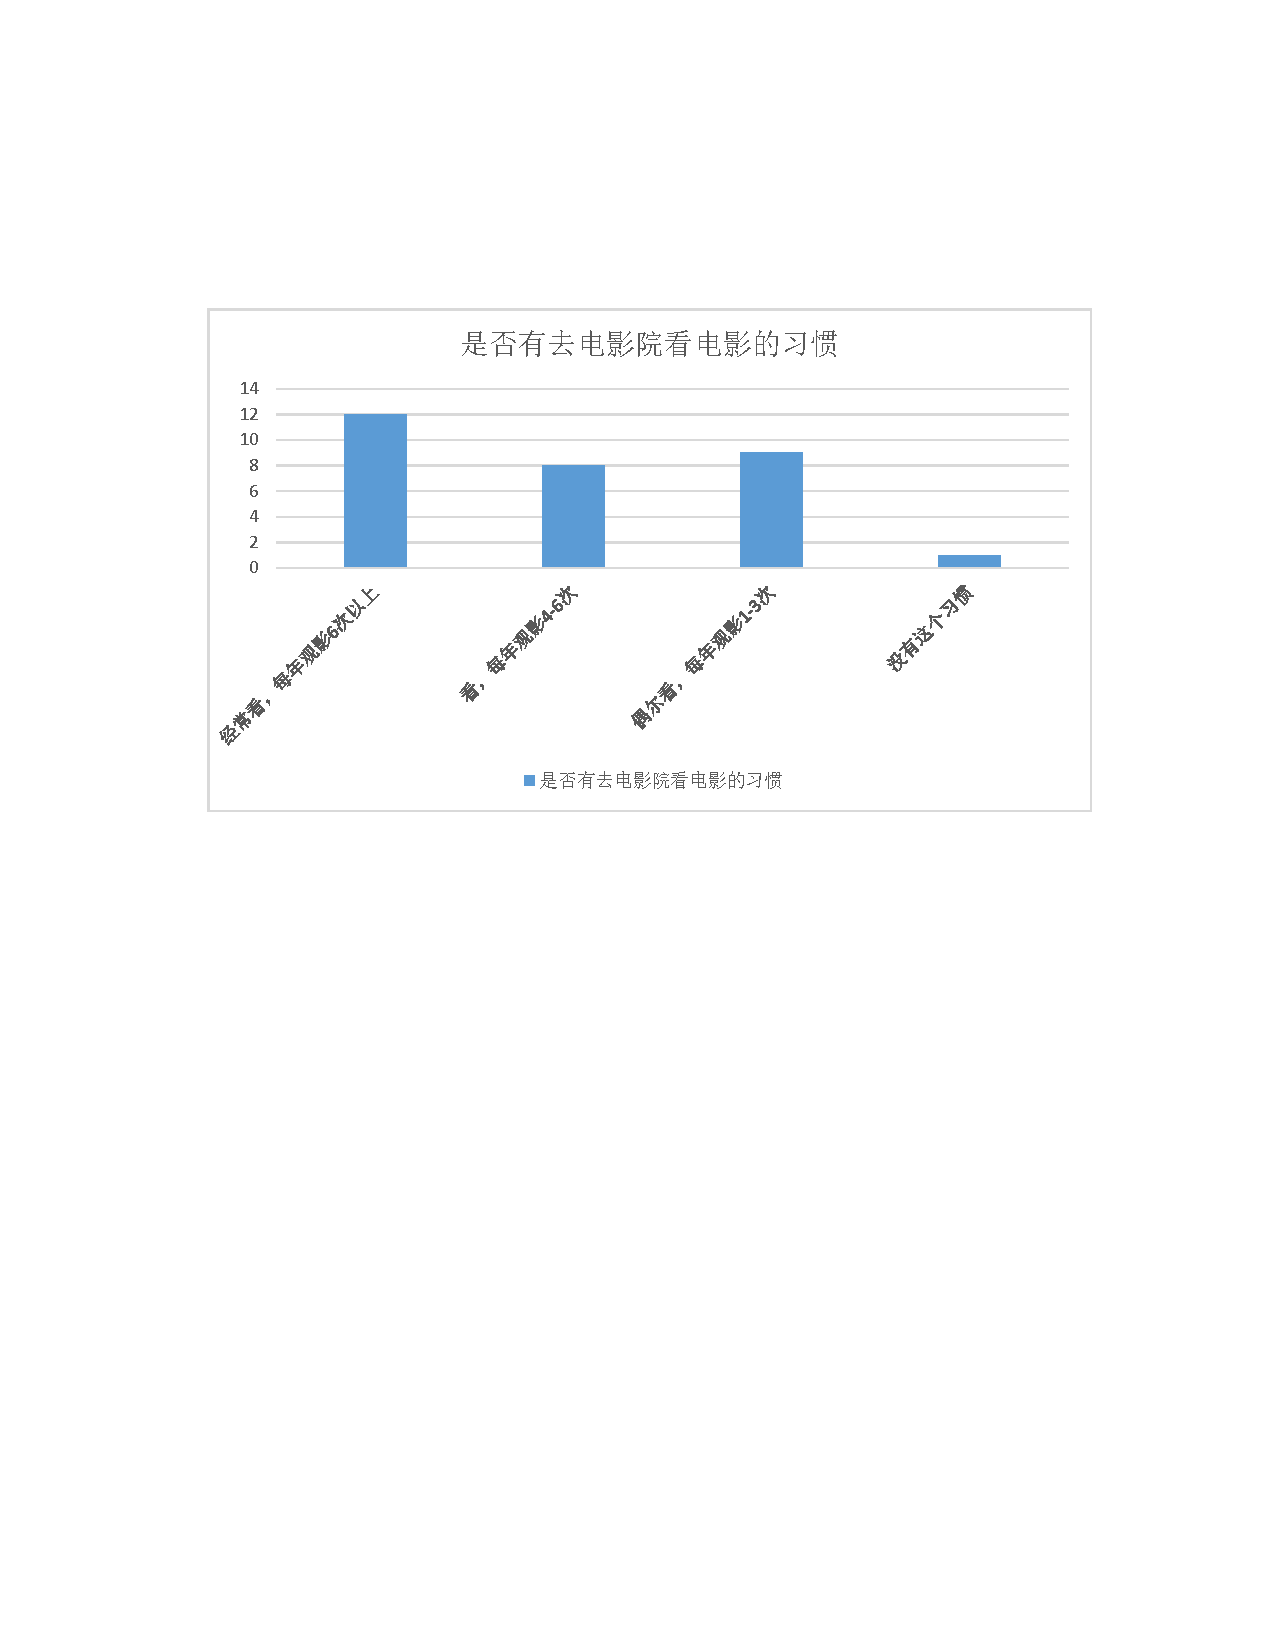
\includegraphics[width=0.6\textwidth]{figure/2.pdf}
\end{figure}
  \item 很明显的可以看出,现在大部分去电影院看电源的人已经开始更加习惯互联网的购票方
式,而且其中在线选座购票的方式更是占了大多数。
\begin{figure}[H]
  \centering
  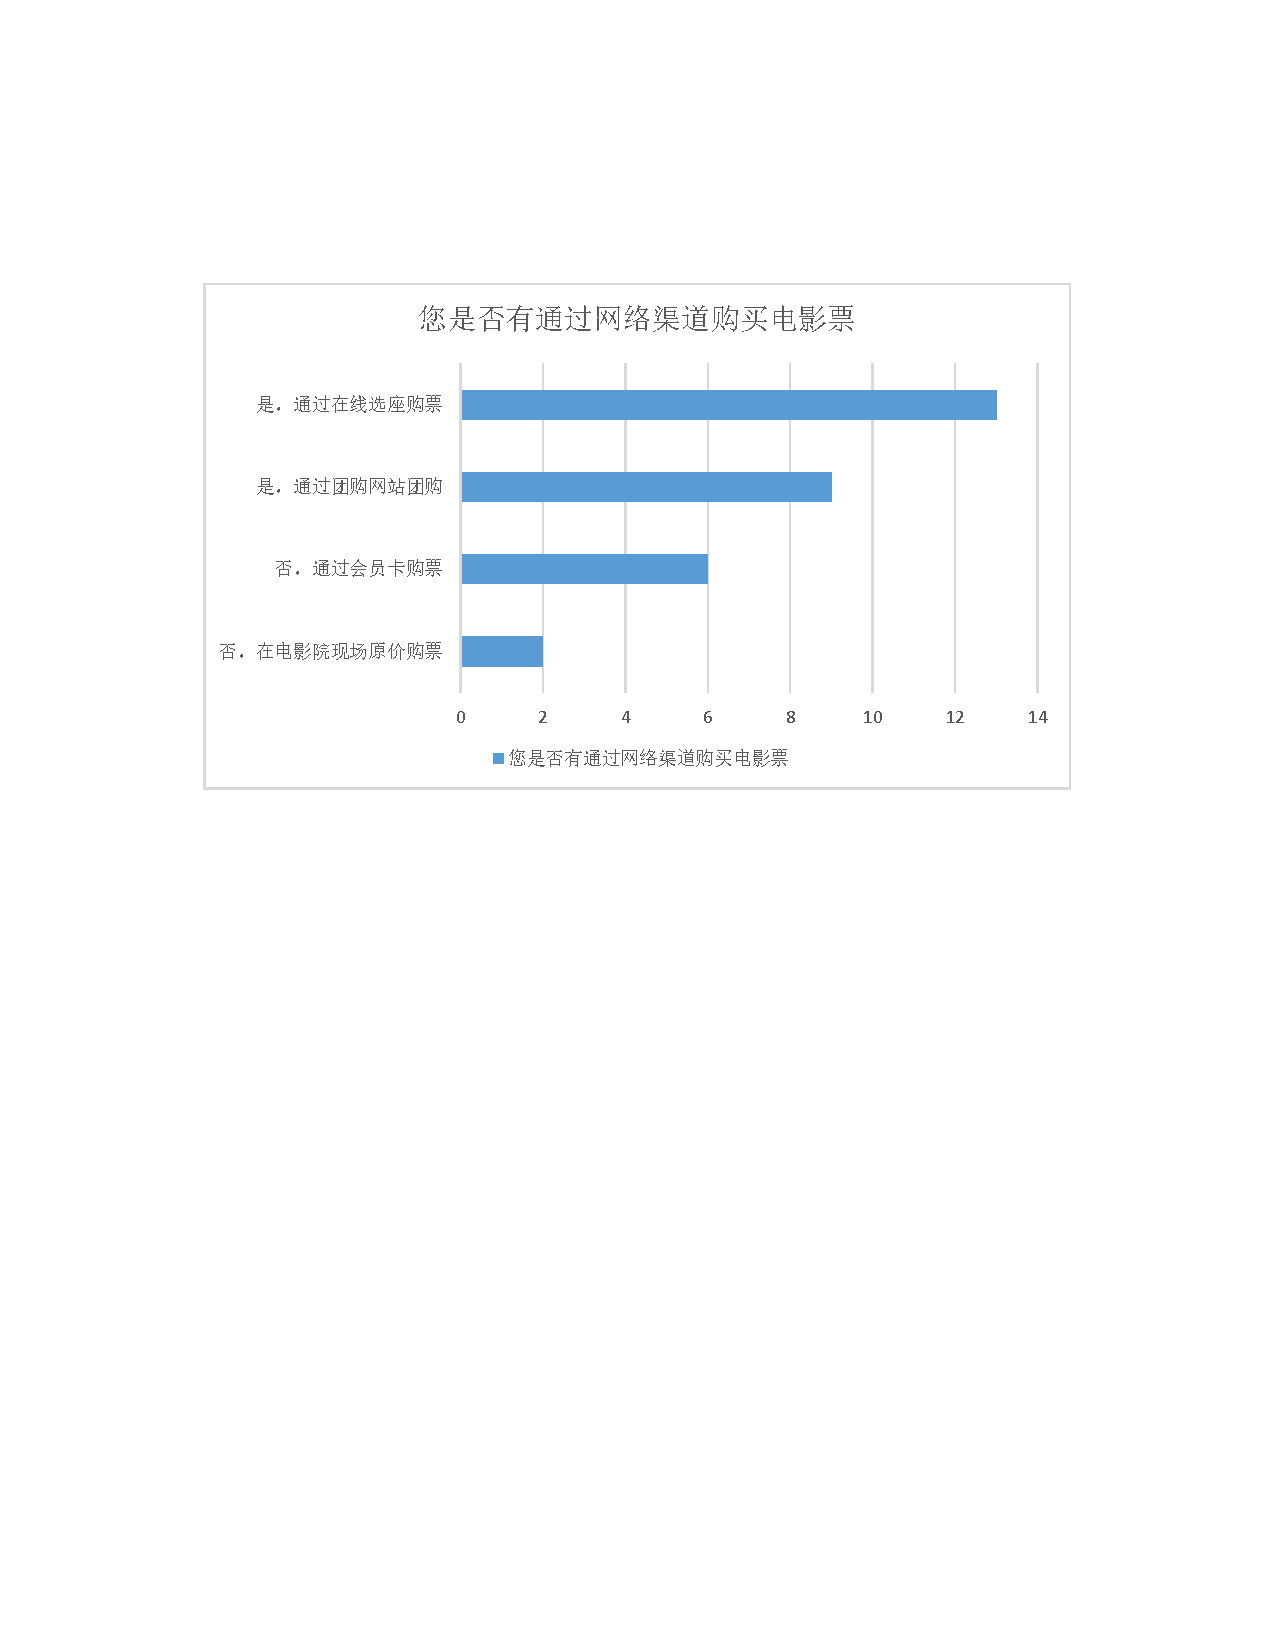
\includegraphics[width=0.6\textwidth]{figure/3.pdf}
\end{figure}
  \item 在这一个问题中,我们可以发现微信和猫眼电影以及大众点评的使用普及度更加高,因
此我们在之后开发的过程中将参照这几款在线电影售票应用,发现他们的优点和可以学习的
地方,在此之上寻求改进和优化的方法。
\begin{figure}[H]
  \centering
  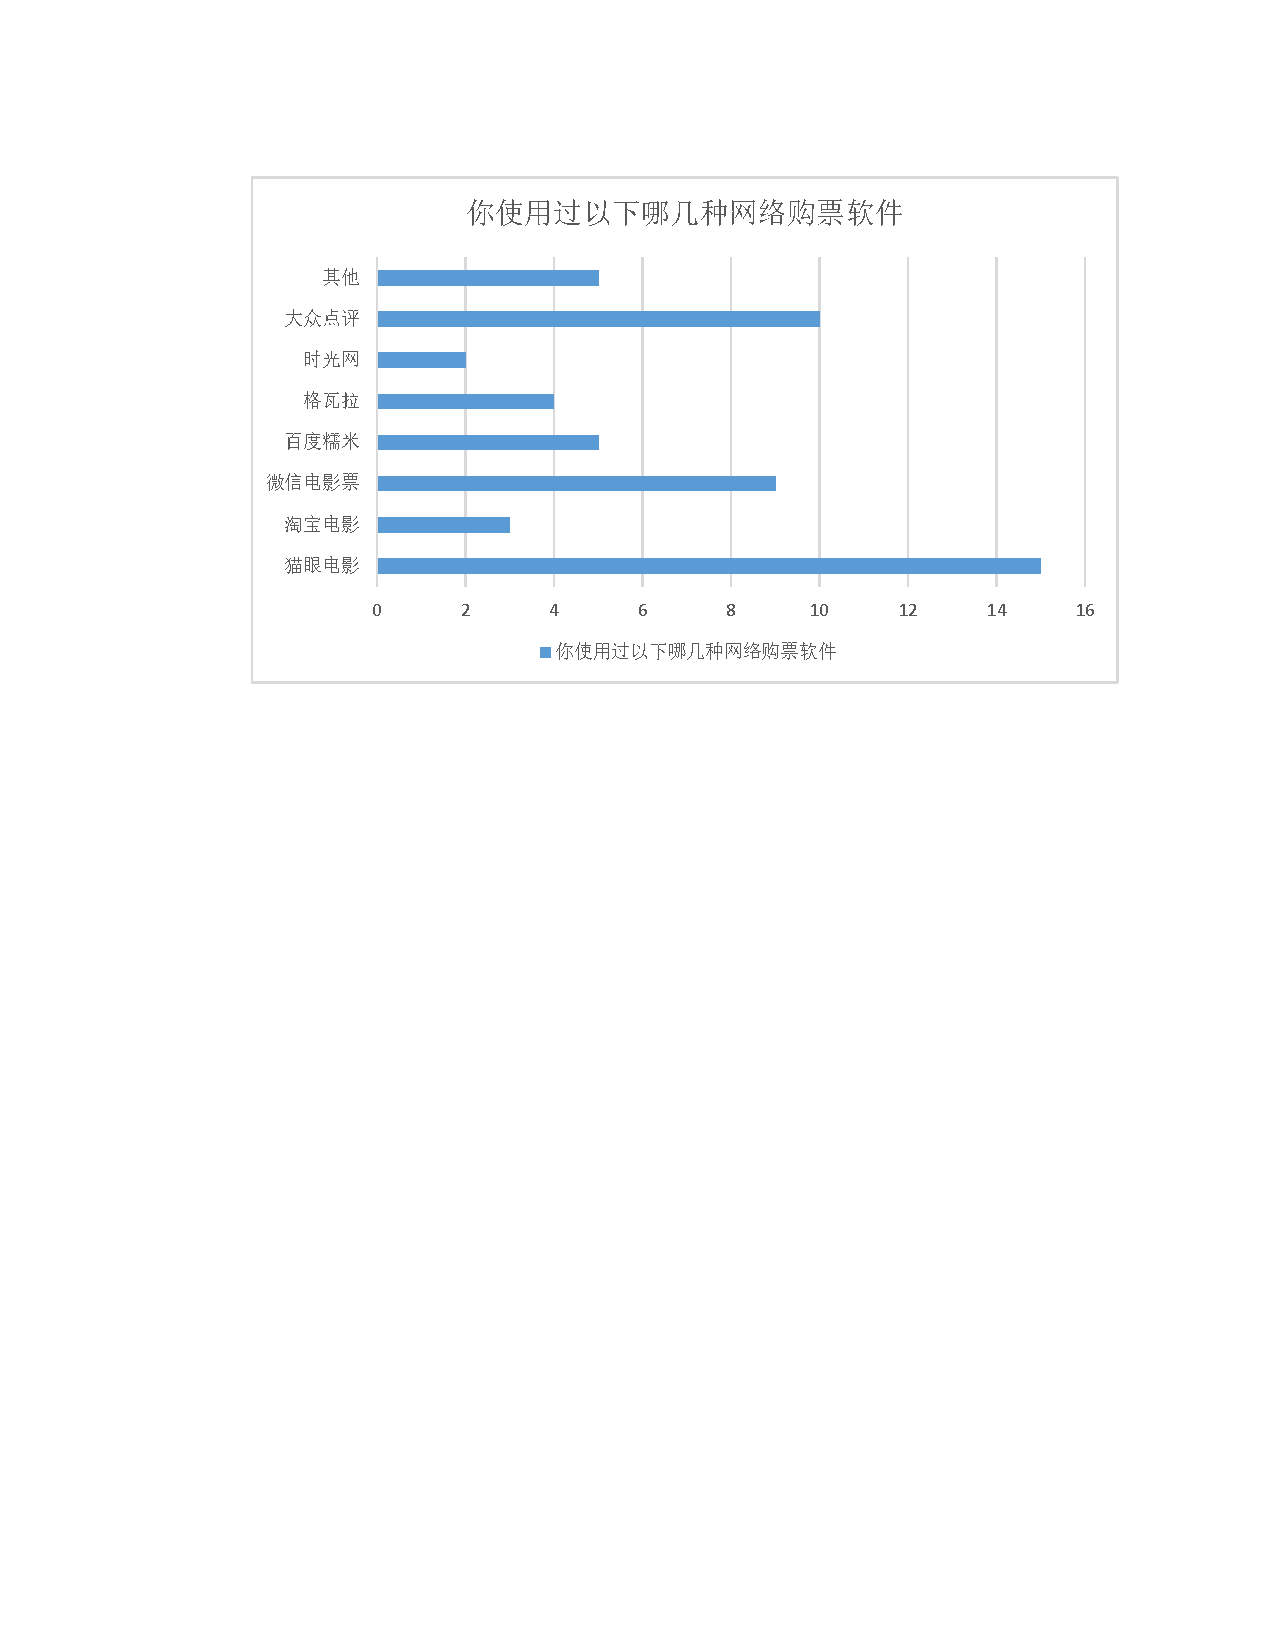
\includegraphics[width=0.6\textwidth]{figure/4.pdf}
\end{figure}
  \item 我们可以发现,对于用户来说,最关心的是电影售票的价格,对于现在的电影售票应用,
因为基本上所有的电影院都会同时在多个软件上售卖自己影院的电影票,因此,用户如果要
去某家电影看电影的话,自然会选择价格更低,或者有优惠促销的软件来购票。
\begin{figure}[H]
  \centering
  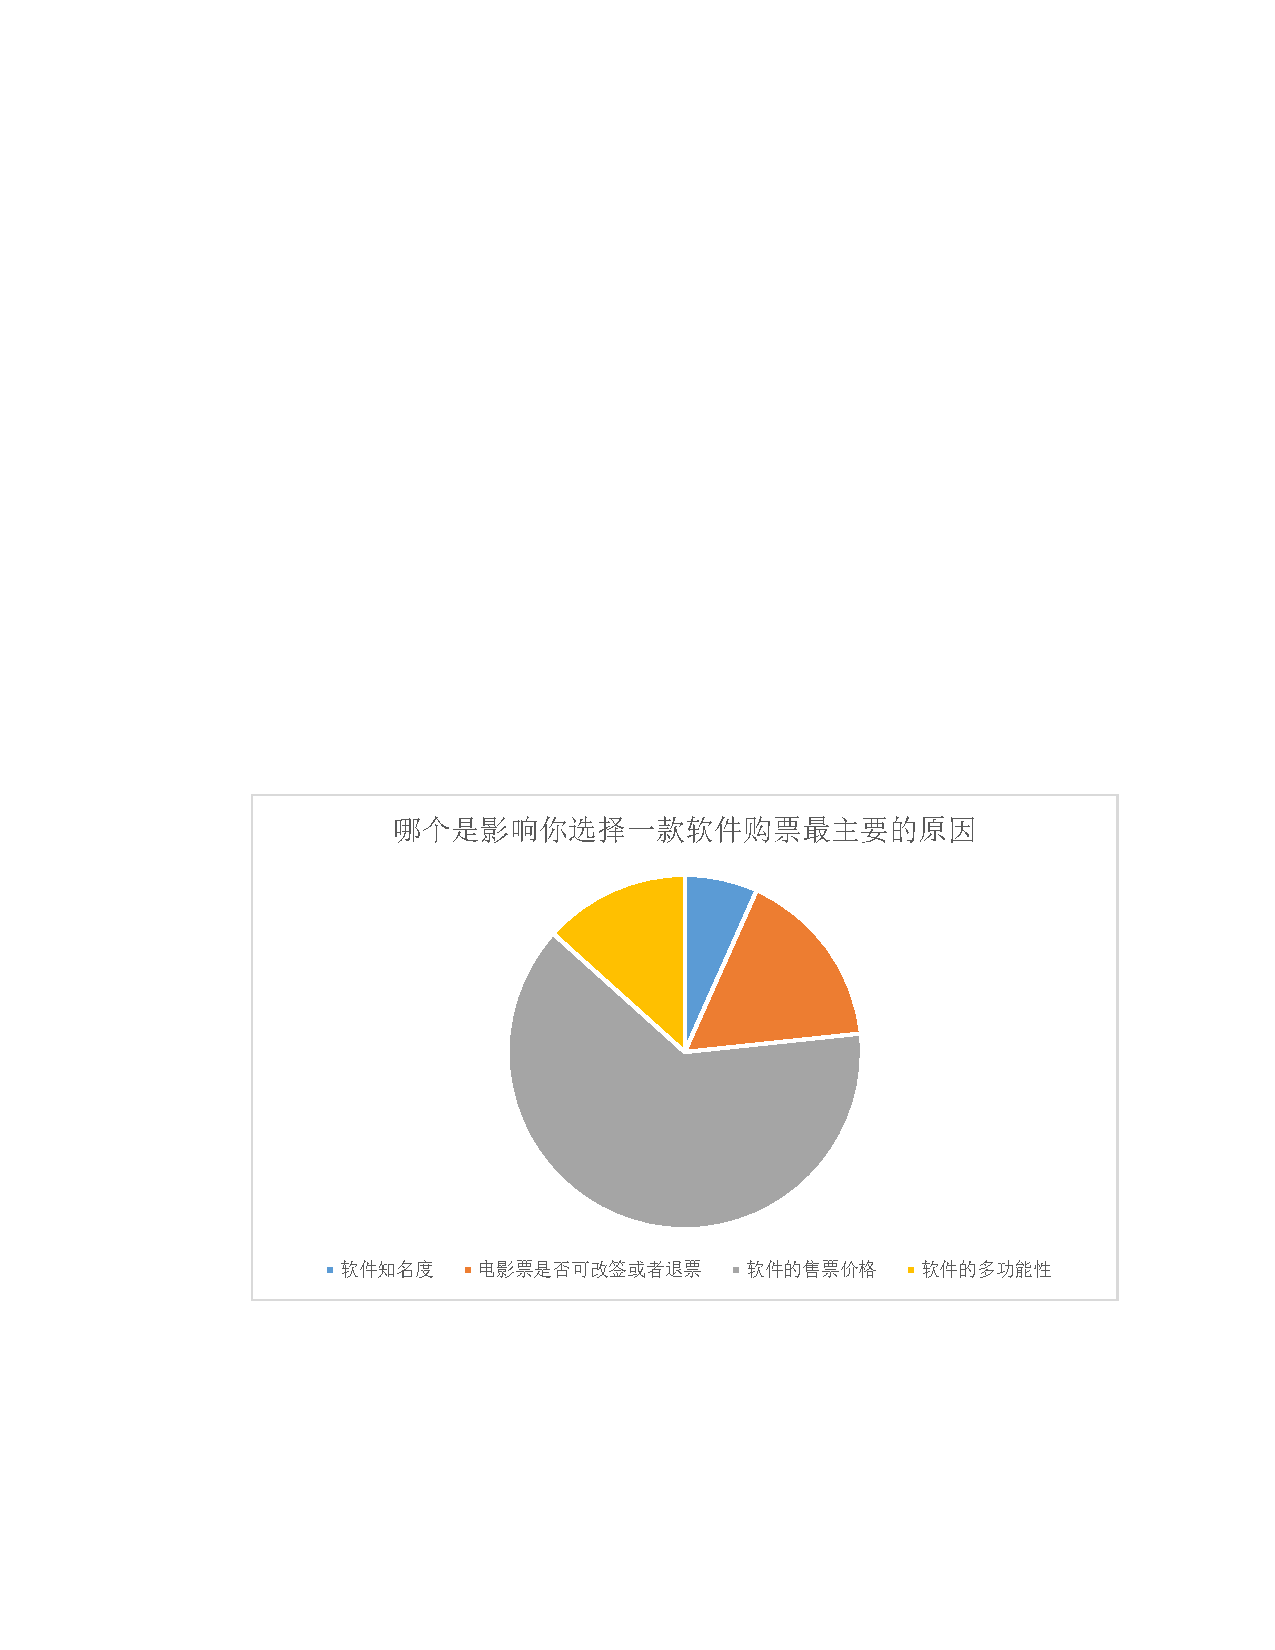
\includegraphics[width=0.6\textwidth]{figure/5.pdf}
\end{figure}
  \item 你最希望现在的在线 电影 购票软件能够添加什么样的功能?
    \begin{enumerate}
      \item 影院室内座位视角图
      \item 查看座位销量
      \item 电影票降价通知
      \item 用户评价与用户购置的座位相关联
    \end{enumerate}
\end{enumerate}

\end{document}
